% labels:
% cap:resultados

% ---------------------------------------------------------------------------- %
\chapter{Resultados}
\label{cap:resultados}
% ---------------------------------------------------------------------------- %

Os resultados foram parcialmente como o esperado.
O agente se saiu muito bem no \textbf{\textit{Gridworld}}, consistentemente encontrando um caminho para o objetivo com diferentes arquiteturas que não fossem drasticamente diferentes.
Já o \textbf{\textit{Pong}} mostrou uma arquitetura bem mais sensível.
Pequenas alterações nos hiper-parâmetros faziam o aprendizado se tornar muito mais lento do que o de costume ou nem acontecer.
Mesmo assim, os resultados se mostraram promissores dado tempo suficiente para o agente treinar e aprender.
O \textbf{\textit{Asteroids}}, por outro lado, não obteve resultados positivos nos vários testes feitos.
Apesar de ser um ambiente propício para o aprendizado por \textit{deep Q-learning}, tendo todas as informações claras na tela, ações bem definidas e recebimento de recompensas simples e consistente, o agente teve grandes dificuldades em conseguir aprender.
Por conta dessas características, esperava-se que ele conseguisse aprender a se comportar nesse domínio, ainda que com dificuldade.

%Todavia, essas observações ainda estão próximos das expectativas.
%O ambiente mais simples, com poucos estados, recompensa e penalidades bem definidos foi o que obteve maior grau de sucesso;
%o de média complexidade dentre os estudados neste trabalho teve resultados promissores;
%e o mais complexo mostrou resultados pouco promissores.

%Ainda que os resultados não sejam muito expressivos, o agente obteve sucesso considerável no \texit{Gridworld}.
%Os hiper-parâmetros escolhidos não foram os melhores, mas foram o suficiente para cumprir o objetivo dos testes.
%
%No \textit{Pong}, a pontuação final é igual a quantidade de pontos do jogador menos a quantidade de pontos do adversário. Como o jogo acaba quando algum dos lados fizer 21 pontos, a pontuação máxima e mínima são 21 e -21 respectivamente.
%Os resultados foram conforme o esperado considerando os artigos lidos sobre o assunto: lento, mas razoavelmente consistente.
%O gráfico abaixo mostra esse crescimento.
%
%\begin{figure}[h!]
%  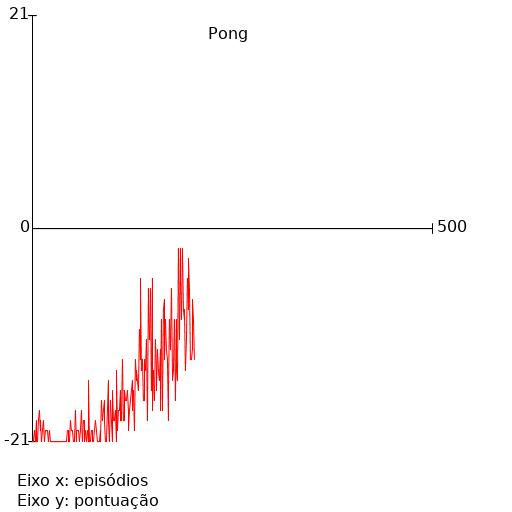
\includegraphics[scale=.5]{pongtuacao}
%  \centering
%  \caption{Pontuação do agente no \textit{Pong} ao longo de 500 episódios de treinamento.}
%\end{figure}

%Testes foram realizados em ambientes mais simples para confirmar o funcionamento do \textit{deep Q-learning} e o quão bem ele se sai em ambientes menos complexos.

%\subsection{\textit{Gridworld}}
%\label{sec:gw}

%O primeiro ambiente foi o \textit{Gridworld}.
%A arquitetura foi testada em três tamanhos de tabuleiro distintos, 5x5, 8x8, e 10x10, todos com armadilhas espalhadas pelo mapa, com algumas diferenças nos hiper-parâmetros para avaliar sua qualidade.
%Nesses três tamanhos, obteve-se uma taxa de sucesso de pelo menos 50\% em 2000 episódios de treinamento.
%Depois disso, o agente foi colocado para percorrer o mapa utilizando apenas política ótima, obtendo sucesso em todos os casos.
%Conclui-se, então, que a arquitetura funciona para ambientes bastantes simples, ainda que tenha sido necessário hiper-parâmetros um pouco mais específicos para cada caso.

%O segundo ambiente testado foi o \textit{Pong}, versão do Atari2600.
%A arquitetura testada teve mudanças maiores quando comparado com feitas entre cada tamanho do \textit{Gridworld}.

%\begin{itemize}
%\item Com tamanho 5x5 e algumas armadilhas espalhadas, o agente teve sucesso em 1212 e fracasso em 788 dos 2000 episódios que jogou.
%\item Com tamanho 8x8 e algumas armadilhas espalhadas, ele teve sucesso em 1034, fracasso em 958 e excedeu o número máximo de ações por episódio em 2 dos 2000 episódios que jogou.
%\item Com tamanho 10x10 e algumas armadilhas espalhadas, teve sucesso em 1458 e fracasso em 542 dos 2000 episódios que jogou, sem haver casos de número máximo de ações por episódio excedido.
%\end{itemize}


%Em ambientes mais simples, como \textit{Gridworld}, o agente conseguiu aprender a chegar no objetivo.
%Sem camadas de convolução, a IA conseguia chegar no objetivo mesmo que estivesse distante.
%Com a adição de camadas ocultas e mais hiper parâmetros para ajustar, foi necessário trazer a recompensa para um espaço mais próximo e mudar as configurações de acordo para se obter sucesso.

%Com esses testes mais simples, foi possível ver a estrutura funcionar, mas o aumento da complexidade do ambiente (matriz de entrada maior, mais elementos para se aprender) fez a dificuldade em encontrar os hiper parâmetros corretos crescer muito mais.
%Além disso, a partir de certo ponto, são necessários centenas de episódios, podendo chegar nos milhares, o que consome muito tempo que não se teve disponível para este trabalho.






%Desde o início da construção da arquitetura da inteligência artificial, diversas alterações foram feitas: mudanças nos hiperparâmetros, no número de camadas de convolução, função de ativação escolhida e técnicas para acelerar aprendizado (\textit{double} e \textit{dueling} descritos acima).
%O melhor resultado obtido foi utilizando os hiperparâmetro descritos \hyperref[table:2]{acima}.
%Jogando sem muito compromisso, consegui 3570 pontos antes de perder todas as vidas e, esforçando-me para obter uma pontuação alta, cheguei em 25130 pontos.
%Logo, o desempenho da IA está bem abaixo do desejado.

